\subsection{House of Quality}
\indent The figure below shows the weighted importance of the project deliverables and their relation to each other. The main marketing requirements are user mobility, user safety, tip-over stabilization, reliability, affordability, and assisted turn. Each of these features are discussed in the previous parts of this document. The main priorities of FORWARD are safety and mobility. 
\\

\begin{figure}[H]
	\centering
	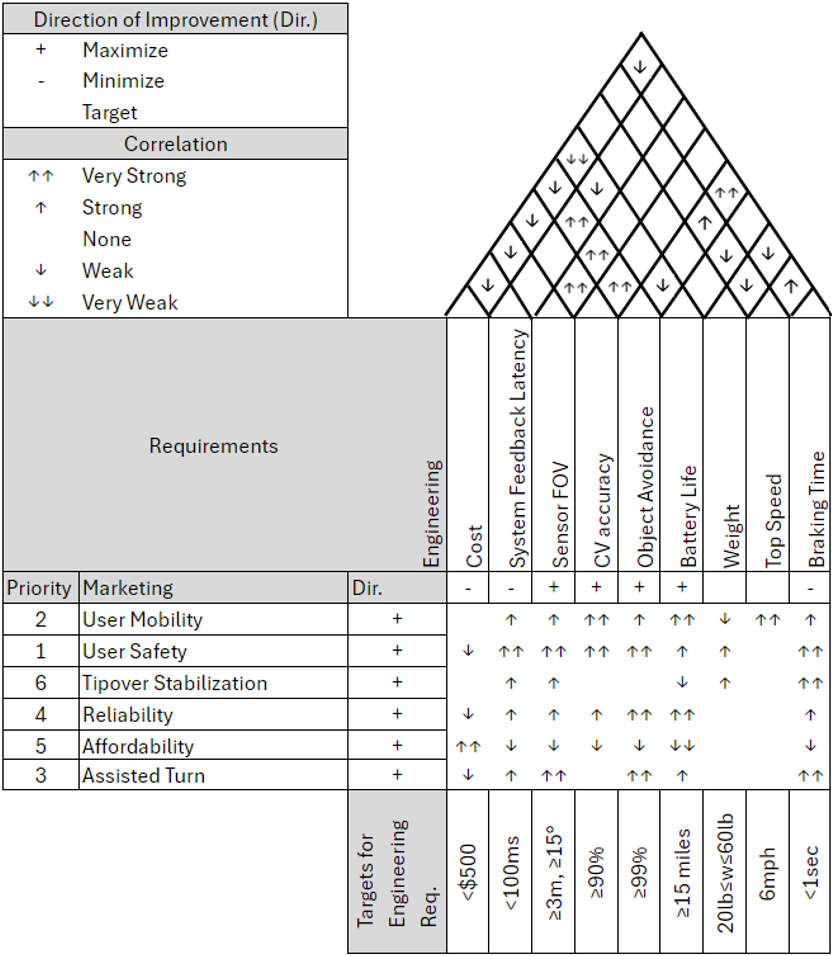
\includegraphics[width=\textwidth]{./Images/HoQ.png}
	\caption{\label{fig:HoQ}House of Quality}
\end{figure}

%\noindent Note that our house of quality diagram roof is diagonally placed. In essence, each diagonal axis is comparing its left neighbor to each other parameter it crosses as it traverses vertically. For instance, the topmost diagonal just under the roof line is comparing cost to system feedback latency, then to sensor FOV, and so on. The next diagonal is comparing system feedback latency to sensor FOV, CV accuracy and so on. \\

\noindent
Note that the engineering requirements from Figure \ref{fig:Standards} are encapsulated on the house of quality as cost, system feedback latency (end-to-end, sensing to user feedback), sensor FOV, CV accuracy, object avoidance (primarily refers to steering protocols), battery life, weight, top speed, and braking time. The ability to efficiently reconcile the marketing requirements with these engineering requirements will spell a great product after design is completed. 
